\documentclass[12pt,conference]{IEEEtran}
%\documentclass[letterpaper,twocolumn,10pt]{article}

\usepackage{graphicx}
\usepackage{url}
\usepackage[usenames]{color}
\usepackage{listings}
\usepackage{wrapfig}
\usepackage{dirtytalk}
\usepackage[caption=false]{subfig}
\usepackage[export]{adjustbox}

\newcommand{\citationneeded}{\textsuperscript{\textit{[CitationNeeded]}}}

%------------------------------------------------------------------------- 
% take the % away on next line to produce the final camera-ready version 
\pagestyle{empty}

%------------------------------------------------------------------------- 
\begin{document}

\title{Continuous Integration of Software Management}


%for single author (just remove % characters)
\author{
{\rm Gautam Kumar, Prof. David Socha}\\
Computing and Software Systems\\
University of Washington Bothell\\
\{gautamk,socha\}@uw.edu
} % end author

\maketitle
\thispagestyle{empty}


\section*{Abstract}
Continuous Integration, A practice where developers integrate 
frequently \cite{stahl_modeling_2014} is considered an integral part of Agile 
development. CI is often thought to be a safety net that prevents developers from deploying broken code to production. 

A similar process and ideology of continual improvement and integration can be applied to Software Management, The art and science of planning and leading software projects \cite{stellman_applied_2005}.

This paper attempts to explore the process of creating such an integration practice within an Organisation.

\subsubsection*{Keywords}

Software Management, Agile development, Continuous Integration

\section*{Introduction}

Martin Fowler in his seminal article \cite{fowler_continuous_2006} on Continuous Integration describes it as a practice where members of a team integrate their work frequently and each integration is verified by an automated build to detect problems quickly.

In the context described above integration is the process of combining the work of all the developers of a project into a cohesive software. On the other hand if considered generically, Integration can be thought of as a practice of combining the work of multiple people and verifying its correctness. Using a similar collective, Continuous integration could be the process of merging the work of multiple people after specific events or set periods of time.

\section*{Evolving Environment}

The outcome of a well managed software organisation are products which provide value to the customer and satisfy their need. In today's fast changing technology landscape the needs and expectations of the customers is always evolving. Such an evolution is affected by various factors, some of which are discussed in the following sections.

\subsection*{Changing customer expectations}

The first few generations of software customers were primarily educational institutions and enterprises where software was merely a means to an end. Customers today, especially in the consumer software market expect an experience rather than just a tool that solves a problem. This explains the reason why organisations today have roles for professionals who work towards streamlining the way people use software \cite{kolko_design_2015} \cite{dixon_stop_2010}.

Customers have also tuned to the idea that organisations which build software systems  are expected to support their products for a long period of time when compared to hardware manufacturers who can get away with launching a new version of their product every year and deprecating old products every 2 years. This could potentially explain the meteoric rise in value of customer support services the market for which is projected to be valued at \$81 billion \cite{wuyts_outsourcing_2015}.

These changes in the customer expectation landscape requires new strategies to be incorporated and verified within the software management process.

\subsection*{New technologies}

Virtual reality, Internet of Things and Machine learning are the hottest consumer technologies evolving as of this writing and all these new technologies promise a new dimension of interactivity and user experience \cite{bachvarov_design-by--customer_2009}. The promise of a new user experience and interactivity comes with added complexity and risk, for example Virtual reality requires new hardware and software capabilities which increases the potential chances of failure and development teams need to evolve new techniques of managing this risk.

\subsection*{Product life cycles and Business models}

Web 2.0 has made a significant impact on the way users and companies buy and sell software. The traditional model of expensive one-time licensing fee has evolved into a small monthly subscription fee and companies are expected to deliver constant updates to their software product. 

A move to the subscription model from the licensing model might require implementing a continuous delivery strategy which might involve simplifying and streamlining the CI system to perform a large number smaller builds rather than single large builds \cite{schief_transforming_2012} \cite{di_valentin_measuring_2012}.


\subsection*{Open source}

Open source software has had a significant impact on the way companies develop software. Open source software helps developers build software faster and enables tapping into the collective wisdom of a larger community of developers. This translates into large savings for companies which is why many organisations are embracing the trend of using open source components within their technology stack \cite{baldwin_4_2014} \cite{lemmens_open_2008}.

Introducing and integrating open source software isn't free, though there is no upfront licensing cost for using open source software. Using open source software requires dedicated effort to adapt to the structure of the software library in question. Security is another concern when using open source software so keeping the system up to date with patches becomes a mandate to preserve the privacy of users and also to fulfil certain legal requirements.

\subsection*{New generation of developers}

A whole new generation of developers have grown up embracing collaborative development techniques such as Q\&A sites, open source software and Hackathons and access or lack thereof to such a community within an organisation may have a significant impact on the productivity of developers \cite{vasilescu_continuous_2014}. 


\subsection*{Effect on Businesses and Software management}

The aforementioned factors can have a significant impact on the projects, people and incidentally the core business of a company. So to achieve business agility and quickly adapt to an ever changing landscape, companies which rely on software technologies need to be able to quickly adapt their software management process \cite{mathiassen_business_2006}.

\section*{Continuous Improvement}

The American Society of Quality define Continuous Improvement to be 
\say{The ongoing improvement of products, services or processes through incremental and breakthrough improvements.} \cite{american_society_for_quality_continuous_????}

Continuous Improvement as a concept has existed for a long time. We can find mentions to continuous Improvement in texts dating back to the mid-19th century \cite{schroeder_americas_????}. 

During the Industrial revolution of the mid-19th century workers were often trained not to think but rather just perform just their task. Thus the task of thinking was effectively cut off from the task of doing, which lead to the thinkers not understanding the practical restrictions of the real world and the increasing complexity of the systems \cite{schroeder_americas_????}. The same concept applies even today with software systems. In large organisations developers are often disenfranchised from the decision making process.

This separation of thinkers from the practical implications of real world lead to the development of Continuous improvement which emphasizes a continuous stream incremental innovation \cite{bessant_rediscovering_1994}.

\section*{Continuous Integration}

Continuous improvement incentivizes a structure where hundreds of people are collectively working on the same basic problem set \cite{bessant_rediscovering_1994}. Continuous improvement brings along with it an explosion of ideas and as some of those ideas implemented a surge in the complexity of the system. Such a surge in complexity eventually leads to either the quality or velocity of development to decline \cite{zaytsev_increasing_2013} . 

Continuous integration thus evolved as a mechanism to manage the risk associated with complex software systems \cite{zaytsev_increasing_2013} and  attempts to provide a safety net \cite{fowler_continuous_2006} to developers. 

Though continuous integration doesn't actually fix bugs, it offers a lot of benefits which help in improving the overall quality of the project such as Improved communication, Project predictability and increased developer productivity \cite{sta_ahl_experienced_2013}. So Continuous integration in many ways can be considered a modern method of complexity control \cite{beck_extreme_2000}.

\section*{Software Management and Continuous Integration}

The inherent complexity in software management is best described by the law of leaky abstractions \cite{spolsky_law_2002} which states that all non-trivial abstractions leak to some degree. 

\subsection*{The Law of leaky abstractions}

An abstraction in the context of computers and software refers to a mechanism that tries to hide the complexity of the underlying system while still offering a useful interface to interact effectively with the underlying system. Abstractions are meant to simplify the process of interacting with an inherently complex system by hiding away certain irrelevant details.

Though abstractions vastly simplify interactions with a complex system, the abstractions are still limited by the capabilities of underlying system and  thus some serious failures always trickle up through abstractions and surprise the user in unexpected ways.

\begin{figure*}
  \centering
  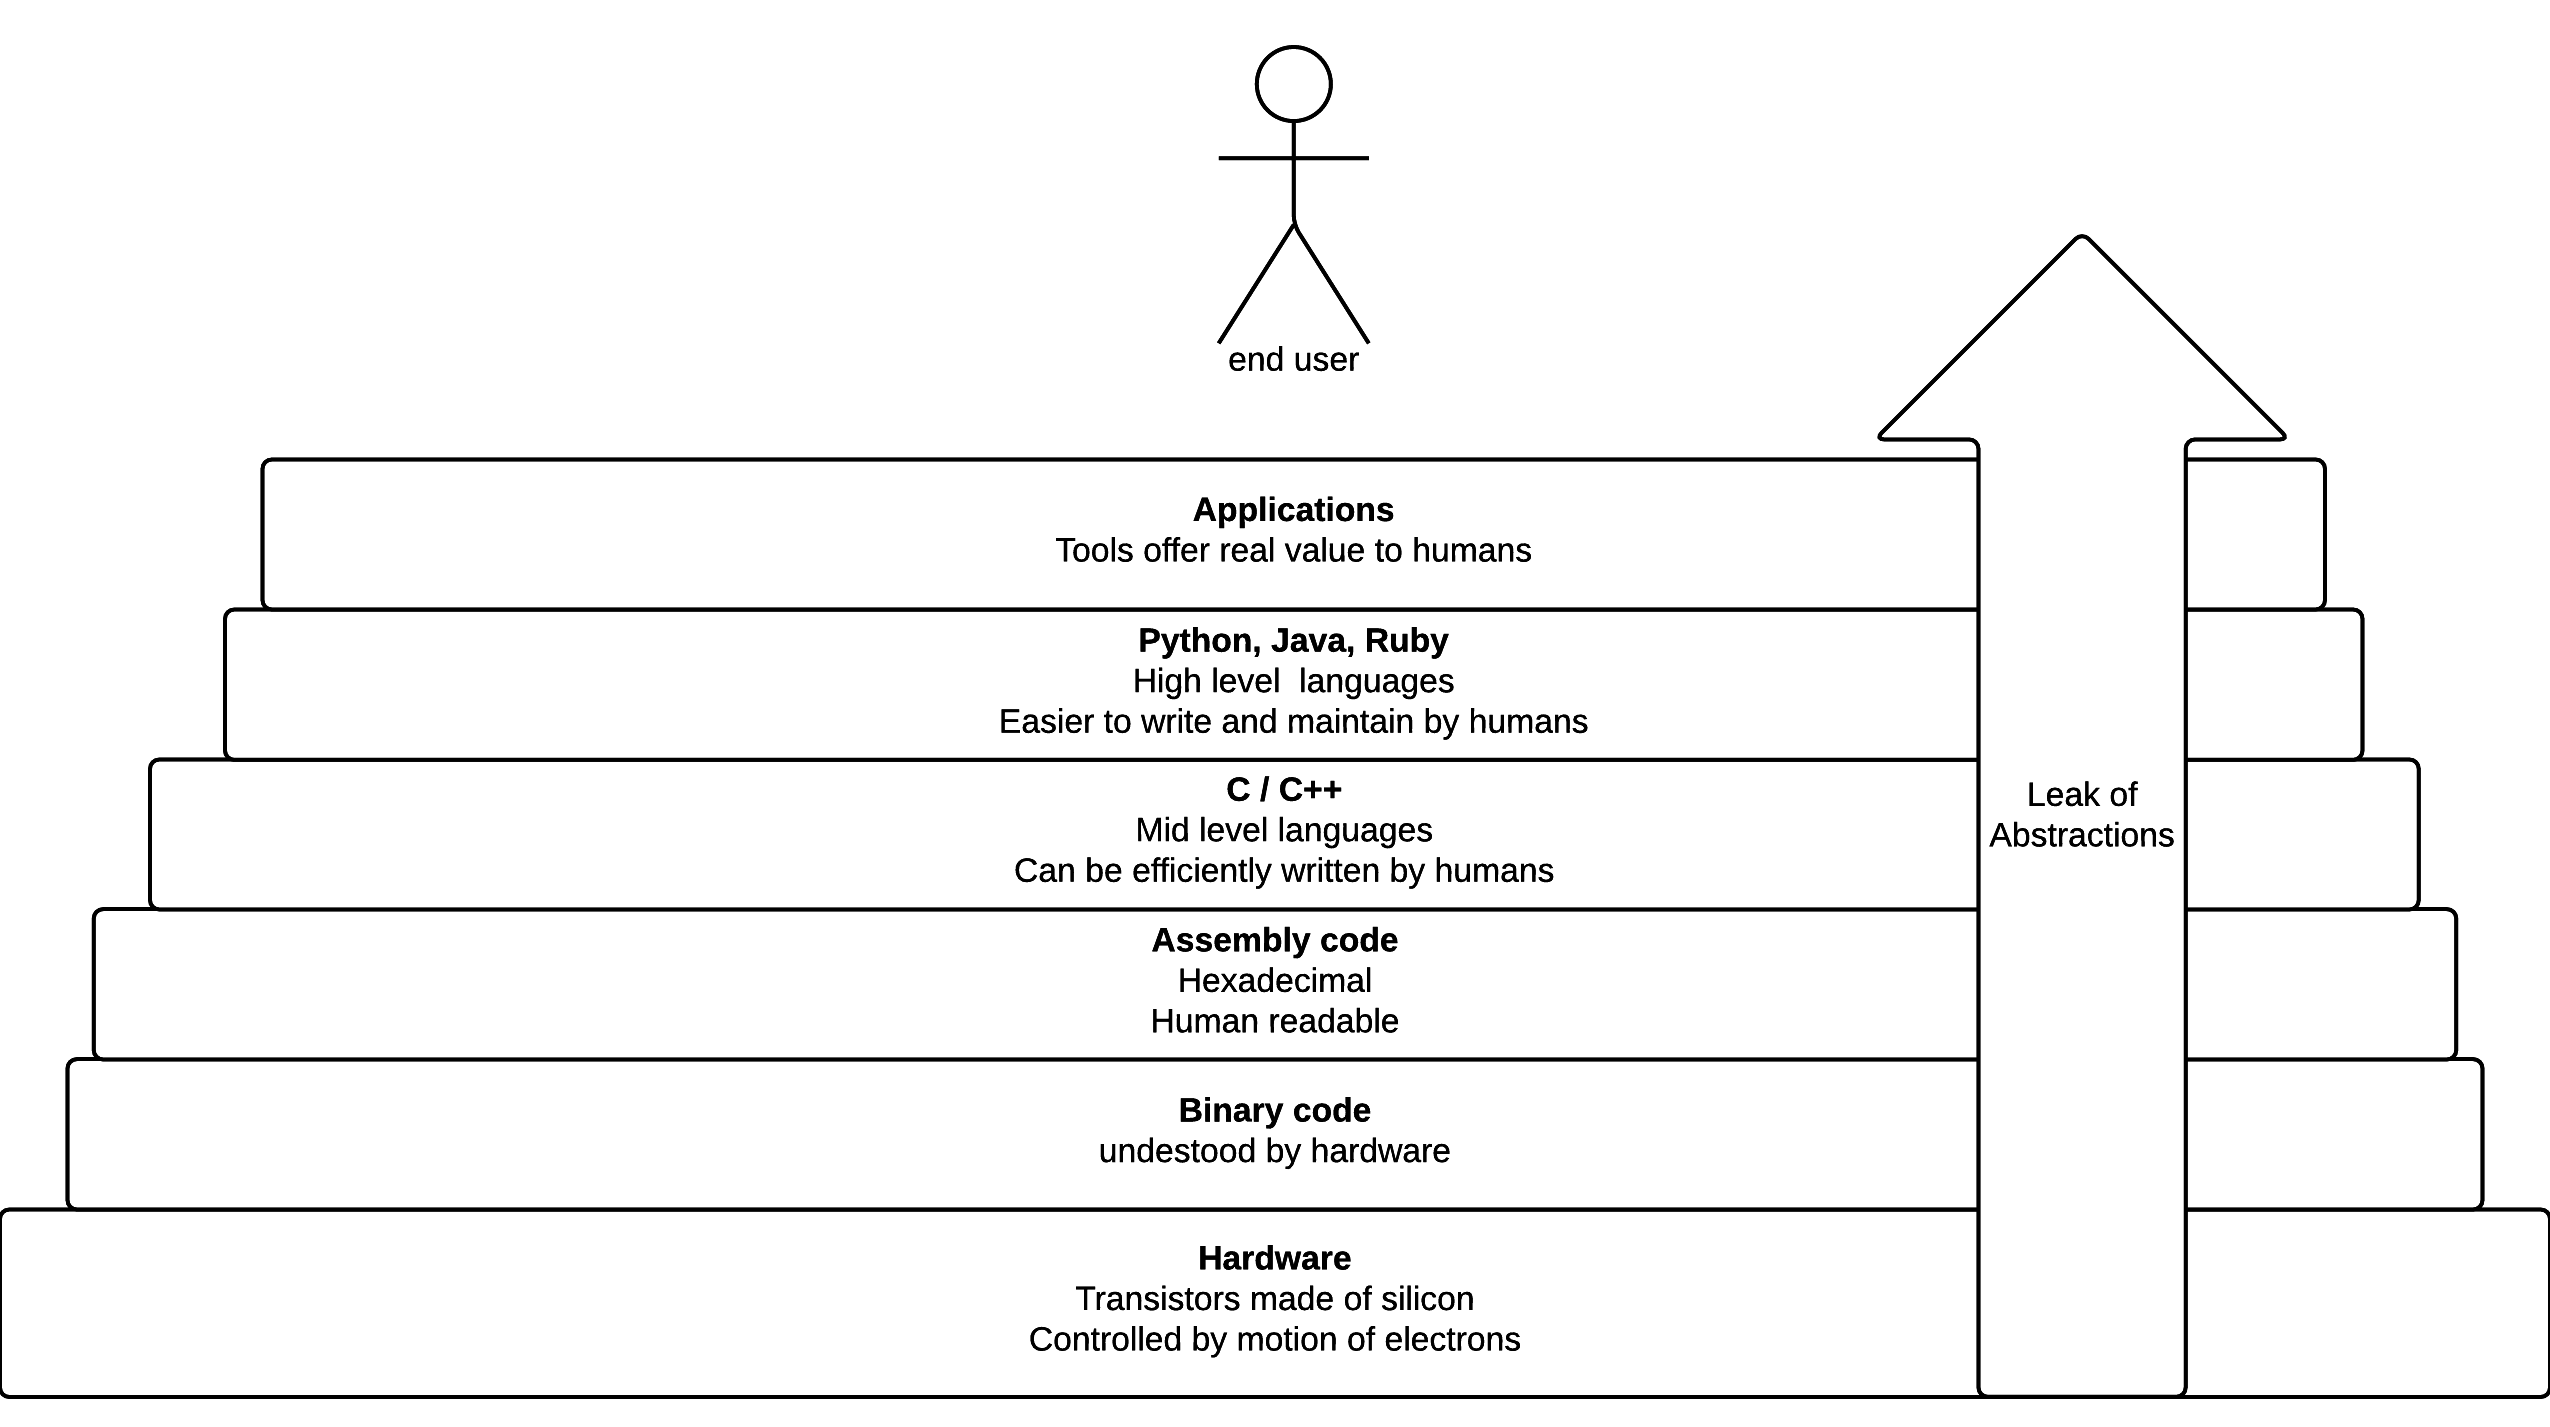
\includegraphics[height=4in]{leakyabstraction}
  \caption{The law of leaky abstraction: All non-trivial abstractions, to some degree, are leaky.}
  \label{leakyabstraction}
\end{figure*}

A classic example of leaky abstractions would be Operating Systems. On the windows operating system any failure in the underlying hardware or its drivers can potentially lead to a BSOD (Blue screen of death) in which the computer displays a cryptic message on a blue screen and prompts the user for action. Though BSOD is a rare occurrence under normal operating conditions, its appearance often perplexes an average user who is unable to make a decision on the next course of action \cite{rosenberg_law_2007}. 

\subsection*{Abstractions in Software Management}

Software Management as a subset of Project management is primarily concerned with balancing the needs of stakeholders with the abilities of developers to deliver value.

Software management practices abstract away the inner workings processes in the organisation. For example Agile methodologies such as Scrum and Kanban are an abstraction which uses best practices from Time management, Team communication, Performance management and Theory of constraints to derive value from developers collaborating within a team. 

Another example of abstraction in Software management in teams would be embracing diversity which is an abstraction over Psychology and Economics to help teams take varied view points on any particular problem. 

\subsection*{CI in Software Management}

Software management is in essence a process which tries to abstract away the chaos of managing an inherently complex task with the help of developers in an ever-evolving environment. As with any non trivial abstraction, software management is leaky and implementing continuous integration into Software management practices could potentially offer benefits similar to software development.



\section*{Scope of Software Management}

The software management process can include areas of management which traditionally come under the purview of Project management such as people management and customer relations. Including these factors into the software management process is however crucial to the overall goal of efficient and effective management of the software process to enable developers to build products that deliver value.

Some potential areas which might come under the purview of software management are

\begin{itemize}

\item People Management
\begin{itemize}
\item Hiring
\item Culture
\item Expectations
\item Organisation structure
\item Diversity
\end{itemize}

\item Project management
\begin{itemize}
\item Requirements gathering
\item Technical choices
\item Project priorities
\item Team selection
\end{itemize}

\item Product management
\begin{itemize}
\item Market analysis
\item Solving the right problem
\end{itemize}

\item Process management
\end{itemize}


\section*{Continuous integration in people management}


Continuous integration has been well defined from the software development perspective, definitions from the side of Software Management on the other hand are quite sparse. 

The value of Continuous integration can only be seen in an organisation that values continuous improvement of the organisation as a whole as opposed to merely using CI as a tool for software development.

The easiest area to define Continuous Integration within the scope of Software management would be Process Management. CI in terms of Process Management could be thought of as a way to verify that all internal processes within an organisation comply with the expectation and solve the intended problem. Some potential implications of a meta-process of Continuous Integration could be weeding out of complicated processes which affect productivity, Simplifying processes to reduce bottlenecks and potentially automation to simplify implementation and verification. There are many tools especially in the BPMN space which offer a simple way to automate and integration internal processes with existing infrastructure. 

\section*{Implementing CI in Software Management}

Continuous Integration and Improvement by nature is an iterative process thus implementing within the context of Software management requires the management team to follow a disciplined process of continuous evaluation and an evolution.

\subsection*{Adoption}
The initial adoption process of any new Software management model would be significantly different from integrating new team members into an existing model. For example, some the factors which affect the success of adopting Agile methodologies in an organisation are 
Customer collaboration, satisfaction and commitment, Communication and negotiation skills of the team and Cultural factors \cite{misra_identifying_2009}.

These success factors differ when brining in new team members. For example a team member fresh out of college might adapt to an existing process at an organisation with ease while a seasoned developer who is loyal to the waterfall model might have a hard time adapting to the rapid pace of an agile organisation. 

As teams being to understand the expectations of their customers and their organisations the previously defined software process evolves thus as time goes on each team / organisation starts building a unique variation of the agile process.

In this context initial adoption is usually the easiest task as the whole team is collectively working towards making sure that Agile adoption succeeds. Adoption by new team members on the other hand depends on the new team member, the Software management team and the culture of the organisation.

It is the responsibility of the software management team to enable new developers to adopt and adapt to the unique process of the dev team they are going to be working with.

\begin{figure}[t]
\centering
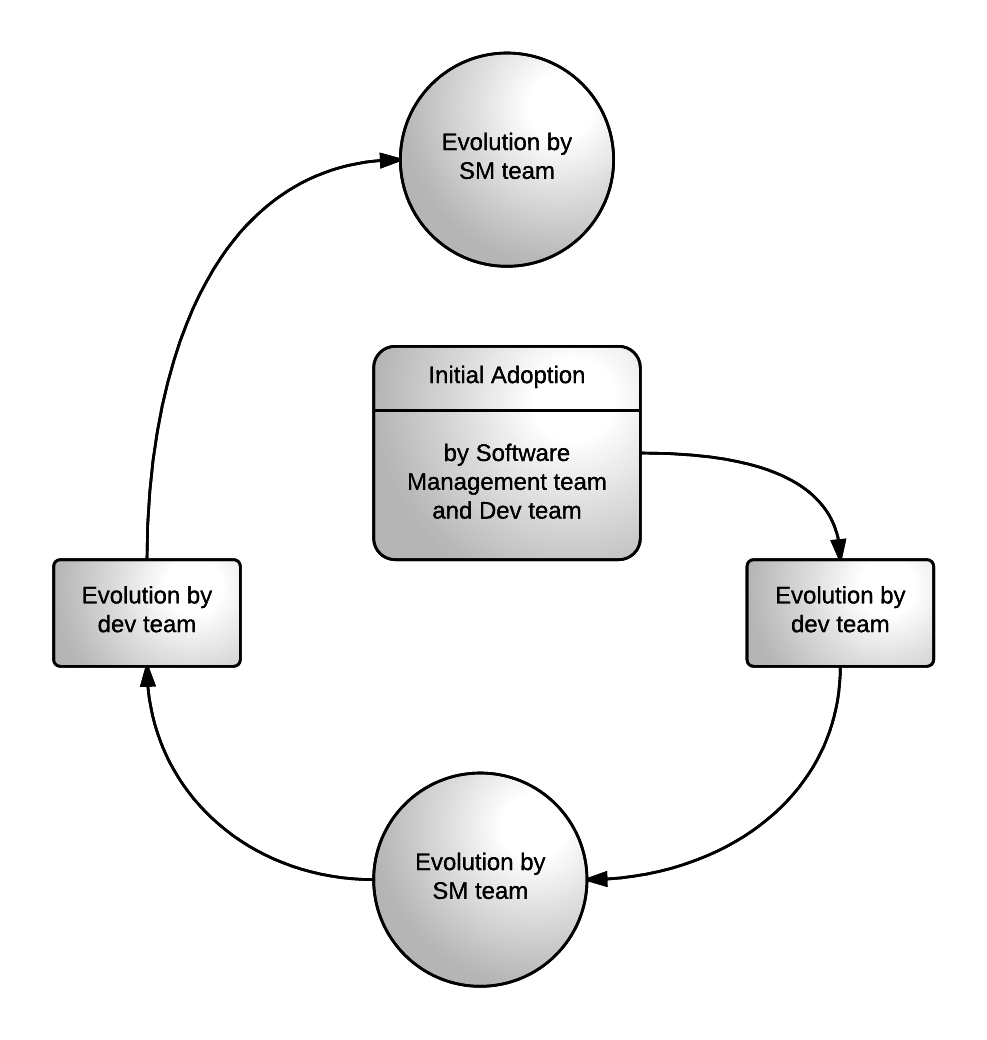
\includegraphics[width=0.4\textwidth]{sm_dev_team_process_evolution.png}
\caption{The Software management team has to evolve the adoption process as the dev team deviates from the initial Software developement model}
\end{figure}

\subsection*{Success criteria} The software management team needs to have a clear and evolving success criteria which monitors the each new hire and how well they are able to adapt to their new teams. This differs from Definition of Done (DoD) based on the fact that DoD is merely a set of activities which need to be performed to get the user story to a shippable state while Success criteria is a broader set of expectations from the candidate which are recorded based on subjective observations. 






\bibliographystyle{plain}
\bibliography{css566_software_management}

\end{document}

